\chapter{Code splitting using dynamic response time modelling}
\label{chap:concepts}

As detailed in Section \ref{sec:double-billing-problem}, serverless functions that interface with external asynchronous services are particularly vulnerable to the double billing problem.

To reduce billed idle time, we propose using code generation to split existing serverless functions around calls to asynchronous services, suspending billing for this period, and resume execution once the asynchronous result is ready.

Since \faaas{} billing is deterministic as described in Section \ref{sec:faas-billing-models}, we can accurately determine the cost of ending an invocation and reinvoking the continuation at a later time. This allows us to build a generic parameterised model described in Section \ref{sec:faas-param-cost-model} that can be applied to any \faas{} platform, given the set of parameters that accurately describe the platform's billing model.

Additionally, in Section \ref{sec:faas-async-service-response-time-modelling} we will introduce a model to estimate response times when interacting with asynchronous services, which in conjunction with the parameterised cost model, will be used to determine the profitability of code splitting in Section \ref{sec:faas-code-splitting-profitability}.

\section{Parameterised cost model for \faas{} platforms}
\label{sec:faas-param-cost-model}

In this section, we will model the costs of invoking serverless functions on a generic \faas{} platform. We will use this model to determine the cost of ending an invocation early and reinvoking the continuation at a later time.

From the billing model described in Section \ref{sec:faas-billing-models}, we can derive a parameterised cost model that generalises across \faas{} platforms. This is model is defined by Equation \ref{eq:faas-billing-model}, which can be is  a function of: a flat-rate invocation cost ($C_i$), and a rate ($C_r$) per unit of time ($G$) charged over the total invocation time ($t$), from the start of a function to the point at which it returns a response, with a minimum billable cost $C_{min}$.

\begin{equation} \label{eq:faas-billing-model}
C(t) \delequal C_i + C_D(t)
\end{equation}

\begin{equation}
C_D(t) \delequal \max\left(C_{min},\ceil*{\frac{t}{G}} C_r\right)
\end{equation}

\section{Asynchronous service response time modelling}
\label{sec:faas-async-service-response-time-modelling}
In this section we will introduce a generic model that is able to estimate the response time of an asynchronous service.

Inherently, network requests and responses are unpredictable due to their asynchronicity. Therefore, it is impossible to directly predict with certainty the response time of an asynchronous service. However, we can model the response time of an asynchronous service as a random variable, and use statistical methods to estimate the expected response time.

Typically, response times are modelled using the 3 parameter Weibull distribution\cite{rouderHierarchicalModelEstimating2005}. The probability density function of the Weibull distribution is given by Equation \ref{eq:weibull-pdf}, where k and $\lambda$ represent the shape and scale parameters respectively, and $\phi$ is the location parameter.

\begin{equation} \label{eq:weibull-pdf}
f(t; k, \phi, \lambda) =
\begin{cases}
\frac{k}{\lambda} \left(\frac{t - \phi}{\lambda}\right)^{k-1} e^{-((t - \phi)/\lambda)^k} & t \geq \phi \\
0 & t < \phi
\end{cases}
\end{equation}

From this probability density function, the cumulative distribution function (CDF) of the Weibull distribution is given by Equation \ref{eq:weibull-cdf}.

\begin{equation} \label{eq:weibull-cdf}
F(t; k, \phi, \lambda) =
\begin{cases}
1 - e^{-((t - \phi)/\lambda)^k} & t \geq \phi \\
0 & t < \phi
\end{cases}
\end{equation}

Given these equations, we can fit a Weibull distribution to the response times of an asynchronous service, as illustrated in Figures \ref{fig:tpch-q2-weibull} and \ref{fig:oltp-q1-weibull}, and use this distribution to estimate the expected response time of the service.

\begin{figure}
    \begin{center}
        \input{node_modules/@faaas-diagrams/db-response-times/assets/tpch-q2-resp-times.pgf}
    \end{center}
    \caption{TPC-H query 2 responses time superimposed with fitted Weibull distribution, executed on a Postgres AWS RDS \texttt{t3.medium} instance called from AWS lambda.}
    \label{fig:tpch-q2-weibull}
\end{figure}

\begin{figure}
    \begin{center}
        \input{node_modules/@faaas-diagrams/db-response-times/assets/oltp-q1-resp-times.pgf}
    \end{center}
    \caption{OLTP bank query 1 responses time superimposed with fitted Weibull distribution, executed on a Postgres AWS RDS \texttt{t3.medium} instance called from AWS lambda.}
    \label{fig:oltp-q1-weibull}
\end{figure}

\section{Function startup and invocation overhead costs}
\label{sec:faas-function-invocation-startup-costs}
In this section we will discuss further the impact of invocation startup costs on the profitability of splitting a function invocation.

When a function is invoked on a \faas{} platform, there are hidden costs associated with the invocation beyond the cost of executing the user's code. These costs are incurred when the function is invoked, and are associated with the setup code that is run before the user's code. This setup code includes the initialisation of the function's execution environment, and the initialisation of the function's runtime.

There has been substantial research into reducing this overhead as described in Section \ref{sec:faas-isolation}, however the overhead has not been completely eliminated, and must be incorporated into models that aim to estimate the cost of invoking a function.

There are two main components to the invocation startup costs: the cold start invocation cost, and the average startup and teardown costs associated with a function invocation.

\subsection{Cold starts}
In the case of cold starts, the function's execution environment must be initialised prior to the function being called. In VM based isolation methods, this involves spinning up a new VM, and loading the function's code into the VM. In container based isolation methods, this involves starting a new container, and loading the function's code into the container. This process can take a non-trivial amount of time, and can be a bottleneck in the performance of a \faas{} platform. This invocation cost is charged to the user. This cold-start invocation cost is a one-off cost, and is not incurred on subsequent invocations of the function, thus for this research, we will not consider this cost in our model.

\subsection{Setup and teardown costs}
The other case is the average startup and teardown costs associated with a function invocation. These costs are incurred on every invocation of the function, and are derived from the setup code that is run before the user's code. This includes establishing connections to databases, and in the context of \faaas{}, writing the result or continuation from executing a handler back to the message queue. These costs are included within the function execution time and so are billed to the customer the same as if it were executing their own code.

Similarly to the response times of asynchronous services, this hidden setup time can be modelled as a Weibull distribution.

\section{Applying code splitting to \faas{} functions}
\label{sec:faas-code-splitting}
In this section, we will introduce the concept of code splitting around asynchronous requests, whereby an existing function is split into two functions, the first making the request, with the second function being invoked by the  asynchronously. This section should give the reader an understanding of the principal behind code splitting.

When performing an asynchronous request in a function, the function will be allocated resources until the request resolves. During this period, the function is billed per unit of time the resources are allocated, rather than by actual usage. During times when the function is waiting for a request to resolve, it is not performing any useful work, and so the user is being billed for idle time.

In a split function, the second handler is invoked with the response when it is ready. This means that after the first function exits, there are no functions executing and so there is no billable time in this period. Whilst in practise this seems benficial, in practise, there are a set of challenges that must be overcome to make this a profitable strategy, most notably the billing model of \faas{} platforms, that charge high invocation costs that negate cost savings made by splitting the function.

\subsection{Continuation passing style}
\label{sec:faas-cps}
Whilst it is possible to run a web server such as ExpressJS inside an AWS Lambda function (and in fact the entrypoint of the AWS Lambda NodeJS runtime does exactly this), the core principal of \faas{} is to abstract away this concept of directly defining the webserver, and instead to execute logic in reponse to an event. As a result, a typical \faas{} function can be considered to have a function signature defined in Type Signature \ref{def:faaas-type-signature}.

\begin{signature}[FaaS Function Handler]
\label{def:faaas-type-signature}
\faas{} functions have type $\textrm{SimpleHandler}$, taking an event and context, and returning a result.

$$\textbf{type}\, \textrm{SimpleHandler} = (\textrm{evt}, \textrm{ctx}) \rightarrow \textrm{result}$$
\end{signature}

This type signature is common across every major \faas{} provider, such as AWS Lambda\cite{amazonAWSLambda2024}, Azure Functions\cite{azureAzureFunctions2024}, Google Cloud Functions\cite{googleGoogleCloudFunctions2024}, OpenWhisk\cite{apacheOpenWhisk2024} and OpenFaaS\cite{ellisOpenFaaS2024}.

This type signature can be augmented such that a function can also return a continuation in addition to a response. This is defined in Type Signature \ref{def:faaas-continuation-signature}.

\begin{signature}[FaaAS Function Handler]
\label{def:faaas-continuation-signature}
A function $f$ or continuation $c$ has type $\textrm{Handler}$ if it returns a type containing either its continuation and context to be reinvoked later, or a result:

$$\textbf{type}\, \textrm{Handler} = (\textrm{evt}, \textrm{ctx}) \rightarrow (\textrm{Handler}, \textrm{ctx}) + \textrm{result}$$
\end{signature}

\faas{} functions of this type can then be executed by an executor defined in Signature \ref{def:faaas-executor} which is responsible for invoking the function with an initial event and context, and then handling the result or continuation.

\begin{signature}[FaaAS Function Executor]
\label{def:faaas-executor}
A function executor $e$ of type $\textrm{Exec}$ is reponsible for invoking a \faaas{} handler of type $\textrm{Handler}$ \textbf{until completion} with an initial event and context, and then returning the result:

$$\textbf{type}\, \textrm{Exec} = (\textrm{Handler}, \textrm{evt}, \textrm{ctx}) \rightarrow \textrm{result}$$
\end{signature}

When function handlers execute asynchronous requests, they return a proxy handler of type $\textrm{Handler}$, which is executed by the proxy itself. Upon completion of the asynchronous request, the proxy handler returns its passed continuation, and the rest of the function handler is executed. This proxy is defined in Signature \ref{def:faaas-proxy}.

\begin{signature}[FaaAS Proxy Handler]
\label{def:faaas-proxy}
A proxy handler $p$ of type $\textrm{Proxy}$ is responsible for invoking a \faas{} handler of type $\textrm{Handler}$ \textbf{until completion} with an initial event and context, and then returning the result:

$$\textbf{type}\, \textrm{Proxy} = \textrm{Handler} \rightarrow (\textrm{evt}, \textrm{ctx}) \rightarrow (\textrm{Handler}, \textrm{ctx})$$
\end{signature}

In practise these continuations are implemented using a message passing system, where the continuation is registered with a message queue, and the context is passed to the continuation when the message is dequeued. This architectural overview is discussed in Chapter \ref{chap:impl}, and illustrated in Figure \ref{fig:faaas-arch}.

\subsection{Avoiding the double billing problem}
In this section, we will illustrate how formalising \faas{} using continuation passing style can be used to avoid the double billing problem described in Section \ref{sec:double-billing-problem}.

The double billing problem arises when a function handler makes an asynchronous request to a service, and then waits for the response. By splitting a single function around an asynchronous request, we can delegate execution of the asynchronous requests to a context with a different billing model, such as Containers-as-a-Service (CaaS), and reinvoke the rest of the function in the original \faas{} context.

To put this into perspective, consider the unsplit function defined in Algorithm \ref{alg:faaas-no-split-example}. In this scenario, a handler \textsc{fst_and_snd} invokes an asynchronous service \verb|sql|, to execute a query. It waits for this query to return before returning the result.

\begin{algorithm}
\caption{Example of a split handler using a proxy}
\label{alg:faaas-no-split-example}
\begin{algorithmic}[1]
\Function{fst_and_snd}{$\textrm{event}, \textrm{context}$}
    \State $query \gets ``..."$
    \State $result \gets \textrm{sql}(\textrm{event})$
    \State \Return $result$
\EndFunction
\end{algorithmic}
\end{algorithm}

This algorithm can be rewritten to use function continuations as shown in Algorithm \ref{alg:faaas-split-example}.

\begin{algorithm}
\caption{Example of a split handler using a proxy}
\label{alg:faaas-split-example}
\begin{algorithmic}[1]
\Function{fst}{$\textrm{event}, \textrm{context}$}
    \State $query \gets ``..."$
    \State \Return \textsc{proxy_db}(\textsc{snd}, $query$, context)
\EndFunction

\Function{proxy_db}{$F', \textrm{query}, \textrm{context}$}
    \State $result \gets \textrm{sql}(\textrm{event})$
    \State \Return $F'(result, \textrm{context})$
\EndFunction

\Function{snd}{$\textrm{event}, \textrm{context}$}
    \State $result \gets \textrm{event}$
    \State \Return $result$
\EndFunction
\end{algorithmic}
\end{algorithm}

In this example, the function \textsc{fst} makes an asynchronous request to a database, and then returns a continuation to a proxy service \textsc{proxy_db}, which in turn invokes the second part of the handler \textsc{snd} before returning the result. The two handlers \textsc{fst} and \textsc{snd} are executed with \faas{}, and the \textsc{proxy_db} handler is executed in a different context, such as a CaaS context. This flow is illustrated in Figure \ref{fig:double-billing-db-split}.

\begin{figure}
    \centering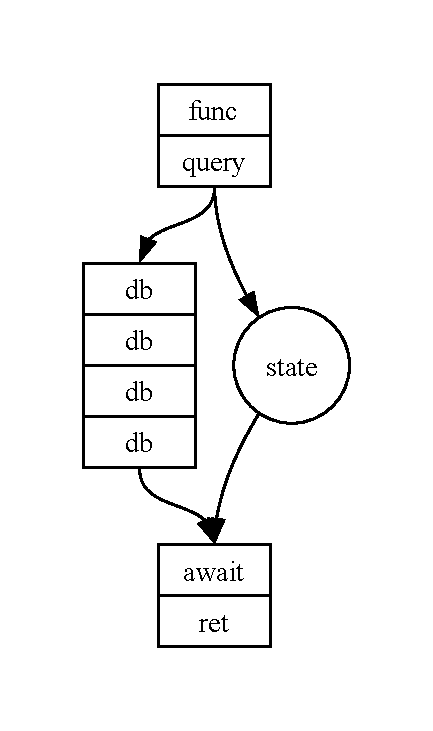
\includegraphics[width=0.75\linewidth]{node_modules/@faaas/double-billing-problem/assets/double-billed-db-split.pdf}
    \caption{Execution a split function querying a database, passing its continuation to the database to execute later.}
    \label{fig:double-billing-db-split}
\end{figure}

\subsection{Continuations as first-class citizens for asynchronous services}
In this research, we have focused on wrapping existing services in proxies, which map the request-response model to a continuation-passing model. This allows us to leverage and test function workloads on existing databases such as PostgreSQL.

By supporting continuations as first-class citizens within existing databases, we would be able to avoid the need to wrap existing services in proxies, and instead invoke the continuation directly from the database, reducing the need to manage and run the proxy service.

This particular concept is referenced later in Chapter \ref{chap:conclusion} under Section \ref{sec:future-work}, where we discuss future work and potential improvements that would improve the performance of \faaas{}.

\section{Capturing Scope}
In this section, we will introduce the concepts behind capturing scoped variables during automatic code splitting to be included in the continuation context.

\subsection{Passing context between continuations}
In order to pass state such as variables between continuations, a context object is passed with a continuation. This context object contains the state of the function at the point of the continuation, and is used by the continuation when it is invoked. This allows the continuation to resume execution of the function, as if there was no split, and to modify variables to be passed to the next continuation or result.

It is important that this context object captures all variables that are required by the continuation, as the continuation will be executed in a fresh execution environment. As a result, the context object must be serializable, as it will be passed between machines.

\subsection{Automatically capturing scope into continuations}
Since from the developer's perspective, the function handler body is a single function, the \faaasc{} compiler must automatically capture variables accessed later from the function handler body at the point of the \verb|'use async'| directive. This is achieved by parsing the function handler body into an Abstract Syntax Tree (AST), and capturing any uses of free variables beyond the split point.

Code can then be generated to capture and serialise any free variables into a context object, and returned with the continuation so that it can be executed with the correct scope. The continuation is invoked when the async request is completed. These free variables are captured using Algorithm \ref{alg:free-variable-analysis}.

\begin{algorithm}
\caption{Free variable analysis for scope capture in continuations}
\label{alg:free-variable-analysis}
\begin{algorithmic}[1]
\Require async directive
\State $V_\mathrm{free} \gets \phi$
\State $V_\mathrm{decl} \gets \phi$

\State $S \gets \textrm{targetOf(async directive)}$

\ForEach {$s \in$ traverseAfter($S$)}
    \If {$s$ is a variable declaration}
        \State $V_\mathrm{decl} \gets V_\mathrm{decl} \cup \{s\}$
    \ElsIf {$s$ is a variable reference}
        \If {$s \notin V_\mathrm{decl}$}
            \State $V_\mathrm{free} \gets V_\mathrm{free} \cup \{s\}$
        \EndIf
    \EndIf
\EndFor
\Ensure $V_\mathrm{free}$
\end{algorithmic}
\end{algorithm}

Once free variable analysis has been performed, the proceeding statements after the async directive can be detached from the AST and reattached to the body for the generated continuation function. This is described in more depth in Section \ref{sec:faaasc-codegen-ast}.

\section{Code splitting profitability analysis}
\label{sec:faas-code-splitting-profitability}
In this section, we will discuss the profitability of splitting a function around an asynchronous request, as defined in Section \ref{sec:faas-code-splitting}, and introduce a model which can be used to determine the probability that splitting a function invocation will be profitable.

As discussed in Section \ref{sec:faas-function-invocation-startup-costs}, there are hidden costs with invoking a function beyond the cost of executing the user's code. This translates into a time penalty incurred when executing a function, where setup code is run before the user's code. This can be formalised into the costing model, by introducing a randomly variable $t_o$ that follows a Weibull distribution shown in Equation \ref{eq:faas-invocation-startup-overhead}, representing the time taken to begin executing a function invocation.

\begin{equation}
\label{eq:faas-invocation-startup-overhead}
t_o \sim \text{Weibull3}(k, \phi, \lambda)
\end{equation}

Using the generic parameterised cost model defined in \ref{sec:faas-param-cost-model}, the total cost of invoking a function, including its overhead, can then be defined as $C_o$ in Equation \ref{eq:faas-cost-with-startup-overhead}.

\begin{equation}
\label{eq:faas-cost-with-startup-overhead}
C_o(t) = C(t + t_o)
\end{equation}

From this total cost, we define an inequality that illustrates the profitability of splitting a function in Equation \ref{eq:faas-split-profitability}. This equation can be rearranged to find a solution for the minimum amount of time that an asynchronous request would need to take for it to be worth splitting the function. This is given by Equation \ref{eq:faas-min-split-time}.

\begin{equation} \label{eq:faas-split-profitability}
C_o(t_0 + t_1 + t_2) > C_o(t_0) + C_o(t_2)
\end{equation}

Since the Weibull distribution is not closed under subtraction, we cannot easily subtract one distribution from another, so we randomly sample $t_o$ as $\hat{t_o}$ from the distribution and use this value to compute a minimum time threshold which a function must be asychronously executing for to decide to split.

\begin{equation} \label{eq:faas-min-split-time}
\begin{aligned}
t_1 > \frac{G}{C_r} \Bigl( & C_D(t_0) + C_D(t_2) \\
& + C_D(\hat{t_o}) + C_i - C_D(t_0 + t_2) \Bigl)
\end{aligned}
\end{equation}

From this we can derive some upper bound heuristics which make it easier to reason about. For example, it is never profitable to split a function if the time saved is less than the equivalent saved invocation cost, as shown in Equation \ref{eq:faas-min-split-time-upper-bound}.

\begin{equation} \label{eq:faas-min-split-time-upper-bound}
t_1 > \frac{G}{C_r} C_i
\end{equation}

Additionally, for platforms that charge a minimum billable cost on function invocations, the decision to split becomes more complex, as the decision to split is also influenced by the expected execution time of the continuation. Consider the pathological but also reasonable scenario where both the initial and continuation sections of a function take less than the minimum billable time to execute, as defined in Equation \ref{eq:faas-min-split-time-pathological-scenario}.

\begin{equation} \label{eq:faas-min-split-time-pathological-scenario}
\begin{aligned}
t_0 + t_2 & < \frac{G}{C_r} C_{min} \\
C(t_0) & = C_{min} \\
C(t_2) & = C_{min} \\
C(t_0 + t_2) & = C_{min}
\end{aligned}
\end{equation}

In this situation, Equation \ref{eq:faas-min-split-time} reduces to Equation \ref{eq:faas-min-split-time-min-cost}, where the minimum time to split must also account for the wasted time in the continuation consumed by the minimum cost ($C_{min}$).

\begin{equation} \label{eq:faas-min-split-time-min-cost}
\begin{aligned}
t_1 & > \frac{G}{C_r} \left( 2 C_{min} + C_i - C_{min} \right) \\
    & > \frac{G}{C_r} \left( C_{min} + C_i \right)
\end{aligned}
\end{equation}

In this section, we will introduce a model to decide profitability of code splitting a function around an asynchronous request. The model is based on the cost/benefit analysis of code splitting, where the cost is the overhead of splitting the function, and the benefit is the reduction in response time.

Using this CDF, we can compute the probability that splitting a function around an asynchronous request will be profitable, given the minimum duration threshold $\hat{t}$. This is given by Equation \ref{eq:faas-split-profitability-weibull}.

\begin{equation}
\hat{t} = \frac{G}{C_r} \left( C_D(t_0) + C_D(t_2) + C_i - C_D(t_0 + t_2) \right)
\end{equation}

\begin{equation} \label{eq:faas-split-profitability-weibull}
\begin{aligned}
P(\mathrm{profit}) & = 1 - F(\hat{t}; k, \phi, \lambda)) \\
P(\mathrm{profit}) & =
    \begin{cases}
    e^{-((\hat{t} - \phi)/\lambda)^k} & \hat{t} \geq \phi \\
    0 & \hat{t} < \phi
    \end{cases}
\end{aligned}
\end{equation}

Using this probability, the function developer can then specify a probability threshold which the function executor can use to determine whether to split the function or not. This model is visualised in Figure \ref{fig:splitting-profitability-analysis-weibull-fit}. In this figure, the Weibull distribution is fitted to the response times of a hypothetical asynchronous request that the system is determining whether to split. The green vertical line at $t = \hat{t}$ represents the minimum time threshold that the function must be executing for in order to overcome the additional invocation cost. The area under the curve to the right of this line represents the probability that splitting the function will be profitable.

\begin{figure}
    \begin{center}
        \input{node_modules/@faaas-diagrams/db-response-times/assets/split-profitability.pgf}
    \end{center}
    \caption{Visualisation of the profitability analysis of code splitting around an asynchronous request, using a Weibull distribution. The green vertical line \^t is the minimum profitability threshold. The green and red areas under the curve represent the probability of profitability and loss by splitting.}
    \label{fig:splitting-profitability-analysis-weibull-fit}
\end{figure}

\subsection{Monitoring and strategy switching}
\label{sec:faaas-monitoring-and-strat-switching-design}
In this section we will discuss how this profitability model can be used to switch between code splitting strategies much more indepth.

Two different splitting strategies are proposed and discussed further in Section \ref{sec:faas-function-splitting-strategies}:

\begin{itemize}
    \item Adaptive splitting
    \item Static splitting
\end{itemize}

In order to effectively perform adaptive splitting as defined in Section \ref{sec:faaas-adaptive-function-splitting}, a response monitor needs to fit a Weibull distribution to the set of response times of the asynchronous request. In order to fit this distribution, the monitor uses Maximum Likelihood Estimation (MLE) to estimate the parameters $k$, $\phi$ and $\lambda$ of the Weibull distribution. These parameters are then used by the function itself to compute the probability of profitability of splitting the function around an asynchronous request.
